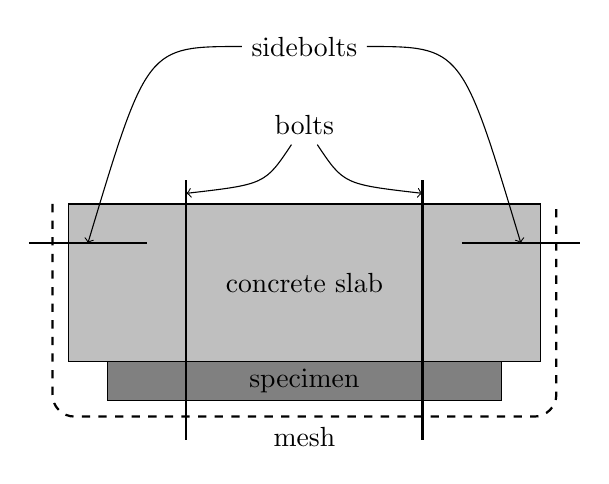
\begin{tikzpicture}
%TOP VIEW OF MESH BOUNDARY

%concrete slab
\filldraw[fill=lightgray] (0,0) rectangle (6,2)
node[pos=.5] {concrete slab};

%sample
\filldraw[fill=gray] (0.5,0) rectangle (5.5,-0.5)
node[pos=.5] {specimen};

%mesh
\draw[thick,rounded corners = 8pt, dashed] (-0.2,2) -- (-0.2,-0.7) -- (6.2,-0.7) node [midway, below] {mesh} -- (6.2,2);

% bolts
\draw[thick]
(1.5,2.3) -- (1.5,-1)
coordinate [pos=0.05] (bolt1)
(4.5,2.3) -- (4.5,-1)
coordinate [pos=0.05] (bolt2);

%sidebolts
\draw[thick] (-0.5,1.5) -- (1,1.5)
coordinate [pos = 0.5] (sbolt1)
(5,1.5) -- (6.5,1.5)
coordinate [pos = 0.5] (sbolt2);

%BOLTS
\draw (3,3) node (bolts) {bolts}
[->] (bolts) .. controls ++ (-0.5,-0.75) .. (bolt1);
\draw [->] (bolts) .. controls ++ (0.5,-0.75) .. (bolt2);

%SIDEBOLTS
\draw (3,4) node (sbolts) {sidebolts}
[->] (sbolts) .. controls ++ (-2,0) .. (sbolt1);
\draw [->] (sbolts) .. controls ++ (2,0) .. (sbolt2);



%what else do I want in here??
%the side bolts
%maybe a sketch of the loom
%pretty graphics anyway

\end{tikzpicture}